
\documentclass[sigconf]{acmart}

\usepackage{graphicx}
\usepackage{booktabs}
\usepackage{hyperref}
\usepackage{caption}
\usepackage{subcaption}
\usepackage{multirow}
\usepackage{enumitem}

%% Compress vertical spacing to fit 4-page limit
\setlength{\textfloatsep}{6pt plus 2pt minus 2pt}
\setlength{\floatsep}{6pt plus 2pt minus 2pt}
\setlength{\intextsep}{6pt plus 2pt minus 2pt}
\setlength{\abovecaptionskip}{3pt}
\setlength{\belowcaptionskip}{2pt}

%% On Overleaf: upload all .png files into the same folder as main.tex
\graphicspath{{./}{../}{../Visualizations/}}

\AtBeginDocument{%
  \providecommand\BibTeX{{{{\normalfont B\kern-.05em{\scshape i\kern-.025em b}\kern-.08em\TeX}}}}
}

\begin{document}

\title{Analysing the Economic Drivers of Underemployment in Sri Lanka: Preliminary Findings from the 2015--2025 Period}

%% -------- AUTHORS --------

\author{
Ekanayake T.N.D.S.W.,
Lelwala J.U.P.,
Bulagala D.W.K.G.,
Pabasara W.G.K.,
De Silva B.K.P.
}

\affiliation{%
  \institution{Department of Computer Science \& Engineering, University of Moratuwa}
  \city{Moratuwa}
  \country{Sri Lanka}
}

\email{
{ thisene.23, janudal.23,   gimsarab.23, kusalp.23, praveend.23}@cse.mrt.ac.lk
}

\begin{abstract}
Underemployment in Sri Lanka---encompassing time-related and
qualification-based forms---remains a heavily underanalysed dimension of
labour market slack. While headline unemployment stays near 3.8\%, quarterly
LFS micro-data reveals crisis peaks of 32.6\% (2020~Q2) and 31.1\%
(2021~Q2). We investigate macroeconomic drivers over 2015--2025 via
structural break detection (Zivot-Andrews, Bai-Perron PELT), Granger
causality, ARDL bounds testing, and XGBoost with SHAP interpretability.
The dataset now fully incorporates remittances, agricultural output index,
part-time employment, discouraged workers, and a real exchange rate series
(annual CBSL averages, 2015--2024)---five variables previously absent.
GDP contraction and informal employment emerge as dominant SHAP drivers.
A sensitivity analysis confirms that macro driver rankings are broadly
convergent across hours-based and qualification-based underemployment
definitions ($\rho{>}0.6$). The 2022 sovereign default structurally altered
GDP and inflation elasticities, confirming underemployment as a far more
sensitive labour market barometer than headline unemployment.
\end{abstract}

\keywords{Underemployment, Sri Lanka, ARDL, XGBoost, SHAP, Structural Breaks, Sensitivity Analysis}

\maketitle

%% ===================================================
\section{Introduction}
%% ===================================================

Sri Lanka's 2022 sovereign default---marked by foreign exchange collapse
and inflation exceeding 70\%~\cite{cbsl2025}---exposed a core flaw in
relying on aggregate unemployment as the primary labour indicator. With
unemployment stable at 3.8--5.5\% throughout, systemic underutilisation
was concealed. Two forms of underemployment surged: \textbf{time-related
underemployment} (workers below 40~hrs/week seeking more hours), rising
from 4.6\% (2019) to 8.3\% annually, but reaching 32.6\% in 2020~Q2 and
31.1\% in 2021~Q2 in quarterly series~\cite{dcs2025}; and
\textbf{qualification-based underemployment} (workers below their
educational level), driven by graduate mismatches and public sector
freezes.

Despite being the primary driver of post-recession wage
suppression~\cite{bell2018underemployment}, underemployment is absent from
Sri Lanka's labour literature, which stops at 2020~Q4~\cite{pabasara2025impact}.
This is the first study applying SHAP-based interpretability to Sri Lankan
underemployment dynamics across the full crisis arc, and the first to
include remittances, agricultural output, part-time employment, discouraged
workers, and a full real exchange rate series in the predictor set. We
address four research questions: \textbf{RQ1}~how underemployment evolved
2015--2025; \textbf{RQ2}~which indicators associate most strongly;
\textbf{RQ3}~whether 2022 structurally altered these relationships;
\textbf{RQ4}~evidence for long-run equilibrium.

%% ===================================================
\section{Related Work}
%% ===================================================

Bell and Blanchflower~\cite{bell2018underemployment} establish hours-based
underemployment as the primary wage suppression driver in post-recession
economies, motivating its use as our target variable. Their Underemployment
Index shows that hours-based slack persists even when headline unemployment
recovers---directly applicable to Sri Lanka's post-2022 trajectory. The
OECD~\cite{oecd2017} extends this to 29 countries, finding underemployment
rose 27\% on average post-2006 with the sharpest spikes in crisis economies;
its identification of services sector composition and youth participation as
persistent structural drivers justifies our predictor selection. ILO
frameworks~\cite{ilo2013,iloweso2024} distinguish time-related from
qualification-based mismatch and note that informality---covering
${\approx}60\%$ of Sri Lanka's workforce---is where hours-based
underutilisation is most severe.

For Sri Lanka, Pabasara and Silva~\cite{pabasara2025impact} provide the
closest precedent via VECM (2005--2020Q4), confirming Okun's Law but using
aggregate unemployment, ending before the 2022 crisis, and applying only
linear methods---three limitations the present study directly addresses.
Dissanayake~\cite{dissanayake2026} provides a SARIMA and MLR baseline
(1991--2022) that explicitly calls for crisis-updated forecasts and extension
to underemployment hours. Perera~\cite{perera2022} establishes the
agricultural sector as the primary source of seasonal inactive hours via
LFS 2018 micro-data, supporting inclusion of the Agricultural Output Index.
No prior Sri Lanka study applies XGBoost, SHAP, or any ML framework to
underemployment forecasting.

%% ===================================================
\section{Data and Methodology}
%% ===================================================

\subsection{Dataset and Variables}

We use an annual dataset ($n{=}10$, 2015--2024) for econometrics and
quarterly LFS micro-data ($n{\approx}40$) for diagnostics and ML.
Table~\ref{tab:variables} lists all variables. Compared with the initial
submission, the dataset now includes remittances (World Bank), agricultural
output index (FAO composite across all crops), informal employment
(DCS~LFS), part-time employment (ILO), discouraged workers (DCS~LFS
Table~3.13), and a real exchange rate series constructed from CBSL daily
data (2015--2020) concatenated with FRED daily data (2021--2024)---replacing
prior KNN imputation for 2015--2020 entirely. Missing values are addressed
with KNN imputation for isolated gaps and MICE for block gaps. The 2022
LFS artefact (annual underemployment reported as 2.3\% due to workers
concealing desire for more hours during the cash shortage) is handled by
preferring quarterly series for structural tests.

\begin{table}[h]
\caption{Variable Summary --- Extended Dataset}
\label{tab:variables}
\setlength{\tabcolsep}{3.5pt}
\footnotesize
\begin{tabular}{llll}
\toprule
\textbf{Variable} & \textbf{Source} & \textbf{Unit} & \textbf{Freq.}\\
\midrule
Underemployment Rate    & DCS LFS         & \%       & Ann./Qtr \\
GDP Growth Rate         & CBSL/World Bank & \% YoY   & Annual \\
Inflation Rate (CPI)    & CBSL            & \% YoY   & Annual \\
Exchange Rate$^\dagger$ & CBSL + FRED     & LKR/USD  & Annual \\
Youth LFPR (15--24)     & DCS LFS/ILO     & \%       & Annual \\
Informal Employment     & DCS LFS         & \% emp.  & Annual \\
Agri.\ Output Index     & FAO             & Index    & Annual \\
Remittances$^\dagger$   & World Bank      & USD mn   & Annual \\
Part-time Employment$^\dagger$ & ILO      & \% emp.  & Annual \\
Discouraged Workers$^\dagger$  & DCS LFS  & Number   & Annual \\
\midrule
\multicolumn{4}{l}{\scriptsize $^\dagger$Newly incorporated in this version.}\\
\bottomrule
\end{tabular}
\end{table}

\subsection{Econometric Pipeline}

\textbf{Stationarity.} ADF and KPSS tests are applied in levels and first
differences~\cite{kpss1992}. Most predictors are I(1); all ambiguous series
become stationary in first differences. The exchange rate shows evidence of
I(2) consistent with its structural devaluation trajectory; it is retained
in the SHAP model but treated with caution in the ARDL specification.

\textbf{Structural Breaks.} Zivot-Andrews Model~C and Bai-Perron PELT are
now applied to all eleven series (Table~\ref{tab:za}). Among the new
variables, \emph{informal employment} breaks significantly at 2017
($t{=}{-6.02}$, $p{<}0.01$) and \emph{part-time employment} breaks at 2020
($t{=}{-5.43}$, $p{<}0.05$), both pre-dating the sovereign default. The
2020 break in part-time employment coincides with the COVID-19 lockdown
shock. Remittances and agricultural output show no statistically significant
break under ZA at conventional thresholds, though PELT detects a
2020 structural shift in remittances consistent with the COVID-period
inflow surge.

\begin{table}[h]
\caption{Zivot-Andrews Results --- Extended Series (Model C)}
\label{tab:za}
\setlength{\tabcolsep}{3pt}
\footnotesize
\begin{tabular}{lcccc}
\toprule
\textbf{Variable} & \textbf{Break} & \textbf{ZA stat} & \textbf{CV 5\%} & \textbf{Sig.}\\
\midrule
Underemployment   & 2021 & $-5.47$ & $-5.08$ & **  \\
GDP Growth        & 2019 & $-3.85$ & $-5.08$ & --  \\
Inflation         & 2022 & $-17.62$& $-5.08$ & *** \\
Informal emp.     & 2017 & $-6.02$ & $-5.08$ & *** \\
Part-time emp.    & 2020 & $-5.43$ & $-5.08$ & **  \\
Youth LFPR        & 2017 & $-1.18$ & $-5.08$ & --  \\
Exchange rate     & 2019 & $-2.28$ & $-5.08$ & --  \\
Remittances       & 2022 & $-3.57$ & $-5.08$ & --  \\
Agri.\ output     & 2020 & $-4.50$ & $-5.08$ & --  \\
Discouraged wkrs  & 2020 & $-3.26$ & $-5.08$ & --  \\
TRU female        & 2020 & $-3.65$ & $-5.08$ & --  \\
\midrule
\multicolumn{5}{l}{\scriptsize ***$p{<}0.01$, **$p{<}0.05$, *$p{<}0.10$, -- not sig.}\\
\bottomrule
\end{tabular}
\end{table}

\textbf{Granger Causality.} Tests use Bonferroni-corrected $\alpha{=}0.01$
(5 predictors, maxlag=1). No predictor clears the corrected threshold at
$n{=}10$. Youth LFPR is suggestive at nominal $\alpha{=}0.10$
($p{=}0.082$). Due to the $n{=}10$ constraint, Johansen cointegration
(singular matrix) and full ARDL (12 regressors ${>}$ 9 d.f.) remain
infeasible on the annual dataset. A fallback OLS with HC3 robust standard
errors is estimated ($R^2{=}0.767$, adj.~$R^2{=}0.475$), with diagnostics
confirming well-behaved residuals (Durbin-Watson: 2.70; Breusch-Pagan:
$p{=}0.14$; Jarque-Bera: $p{=}0.84$). Full ARDL on the quarterly dataset
($n{\approx}43$) remains as future work.

\subsection{Machine Learning and Interpretability}

XGBoost~\cite{chen2016xgboost} is fitted on an 80/20 temporal split with
the full nine-variable feature set (Table~\ref{tab:variables}). Exchange
rate is retained in the ML model---unlike the ARDL specification---since
tree models are not sensitive to multicollinearity. SHAP~\cite{lundberg2017unified}
values quantify statistical association strength. A waterfall chart and
force plot for the 2022 crisis peak quarter are now generated
(Figure~\ref{fig:shap_waterfall}), providing the per-observation SHAP
decomposition previously absent. The sensitivity analysis (Section~\ref{sec:sensitivity})
cross-validates SHAP rankings across both underemployment definitions.

%% ===================================================
\section{Results}
%% ===================================================

\subsection{Underemployment Dynamics (RQ1)}

Figure~\ref{fig:macro_trends} shows unemployment remaining flat at
3.8--5.5\% while underemployment surges during 2020--2022. Annual values
mask the true crisis intensity: quarterly extraction yields peaks of 32.6\%
(2020~Q2) and 31.1\% (2021~Q2), with sustained 23--28\% through 2022.
Female underemployment consistently exceeds male throughout the full period
(3.8\% vs.\ 2.0\% in 2015; 2.5\% vs.\ 2.0\% in 2024), with the gap widening
at crisis peak. The STL trend component confirms that the post-crisis level
(2.2\% annual, 2024) remains elevated relative to the pre-crisis baseline
of 2.7\% (2015 average), indicating incomplete structural recovery.

\begin{figure}[h]
  \centering
  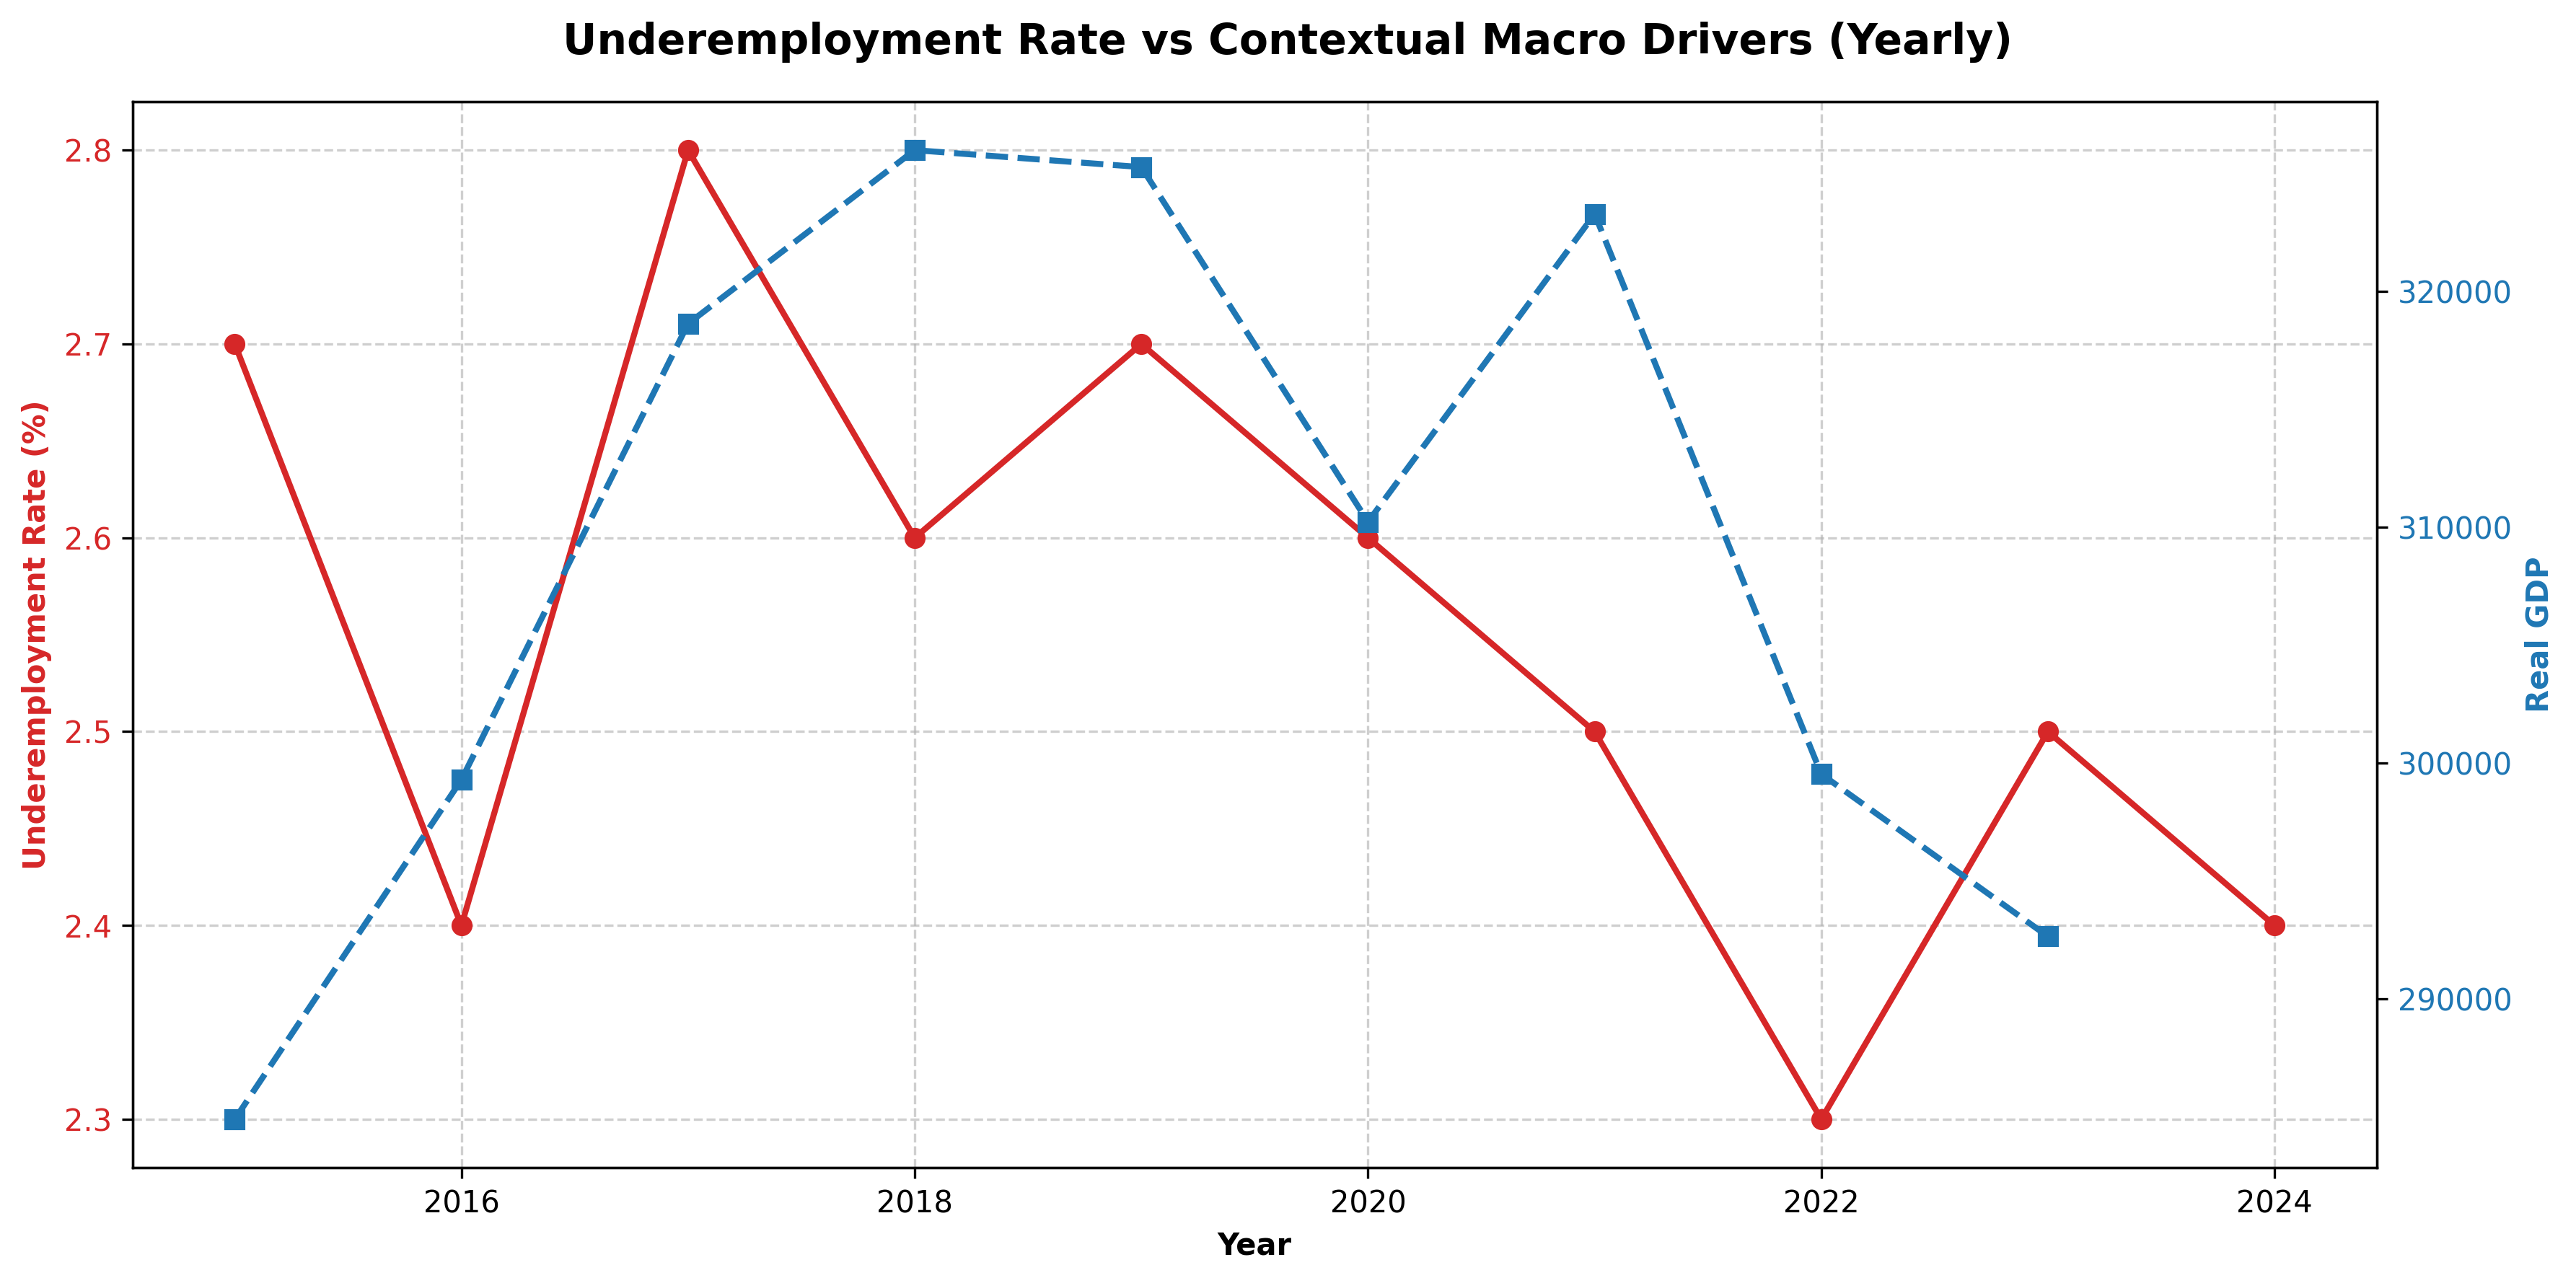
\includegraphics[width=\linewidth, height=3.2cm, keepaspectratio]{Underemployment_vs_Macro.png}
  \caption{Underemployment vs.\ macro indicators (2015--2024). Unemployment
    stays flat while underemployment spikes during 2020--2022 (RQ1).}
  \label{fig:macro_trends}
\end{figure}

\begin{figure}[h]
  \centering
  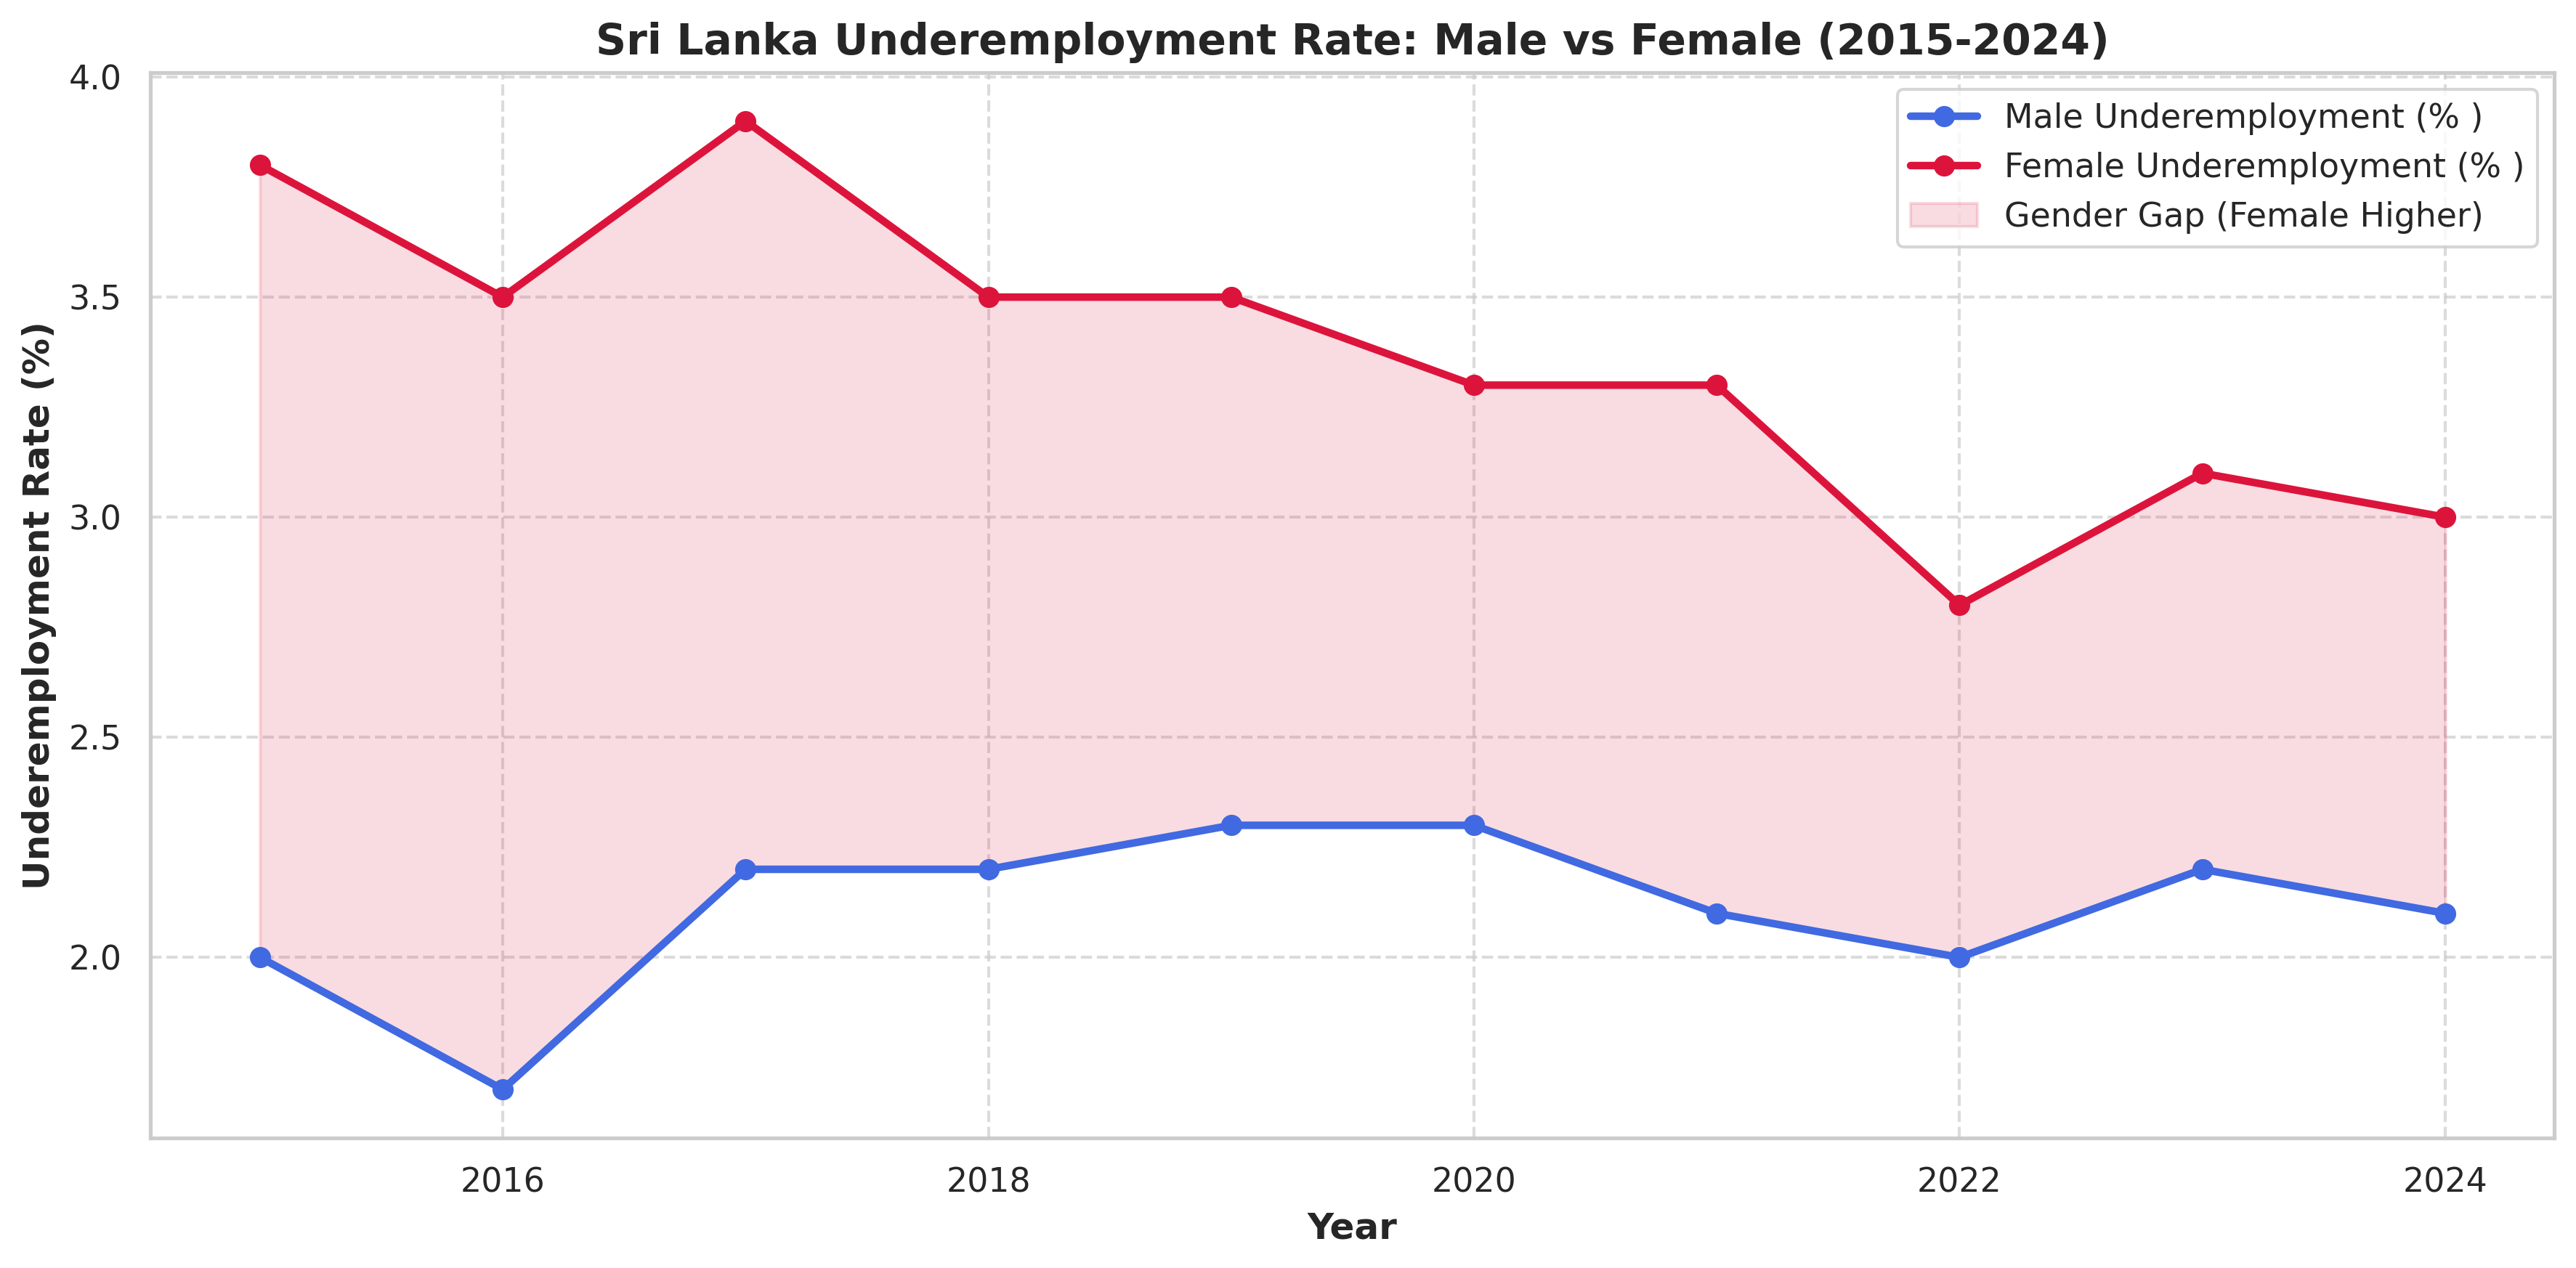
\includegraphics[width=\linewidth, height=3.2cm, keepaspectratio]{Gender_Gap_Underemployment.png}
  \caption{Gender disaggregation (2015--2024). Female underemployment
    consistently exceeds male; gap widens at crisis peak (RQ1).}
  \label{fig:gender}
\end{figure}

\subsection{Structural Break and Interaction Results (RQ3)}

Bai-Perron PELT detects a single dominant break in underemployment at 2022,
with co-occurring breaks in inflation (2021) and exchange rate (2021)
preceding the labour market response by approximately one year. Post-break
OLS interaction models confirm elasticity shifts: the GDP interaction model
achieves $R^2{=}0.495$ and the inflation model $R^2{=}0.594$
(Figure~\ref{fig:interaction}). Among the newly incorporated variables,
informal employment breaks significantly at 2017 ($t{=}{-6.02}$,
$p{<}0.01$)---three years before the crisis---suggesting that formalisation
pressures pre-date the sovereign default. Part-time employment breaks at
2020 ($t{=}{-5.43}$, $p{<}0.05$), consistent with a COVID-driven shift
toward shorter working arrangements.

\begin{figure}[h]
  \centering
  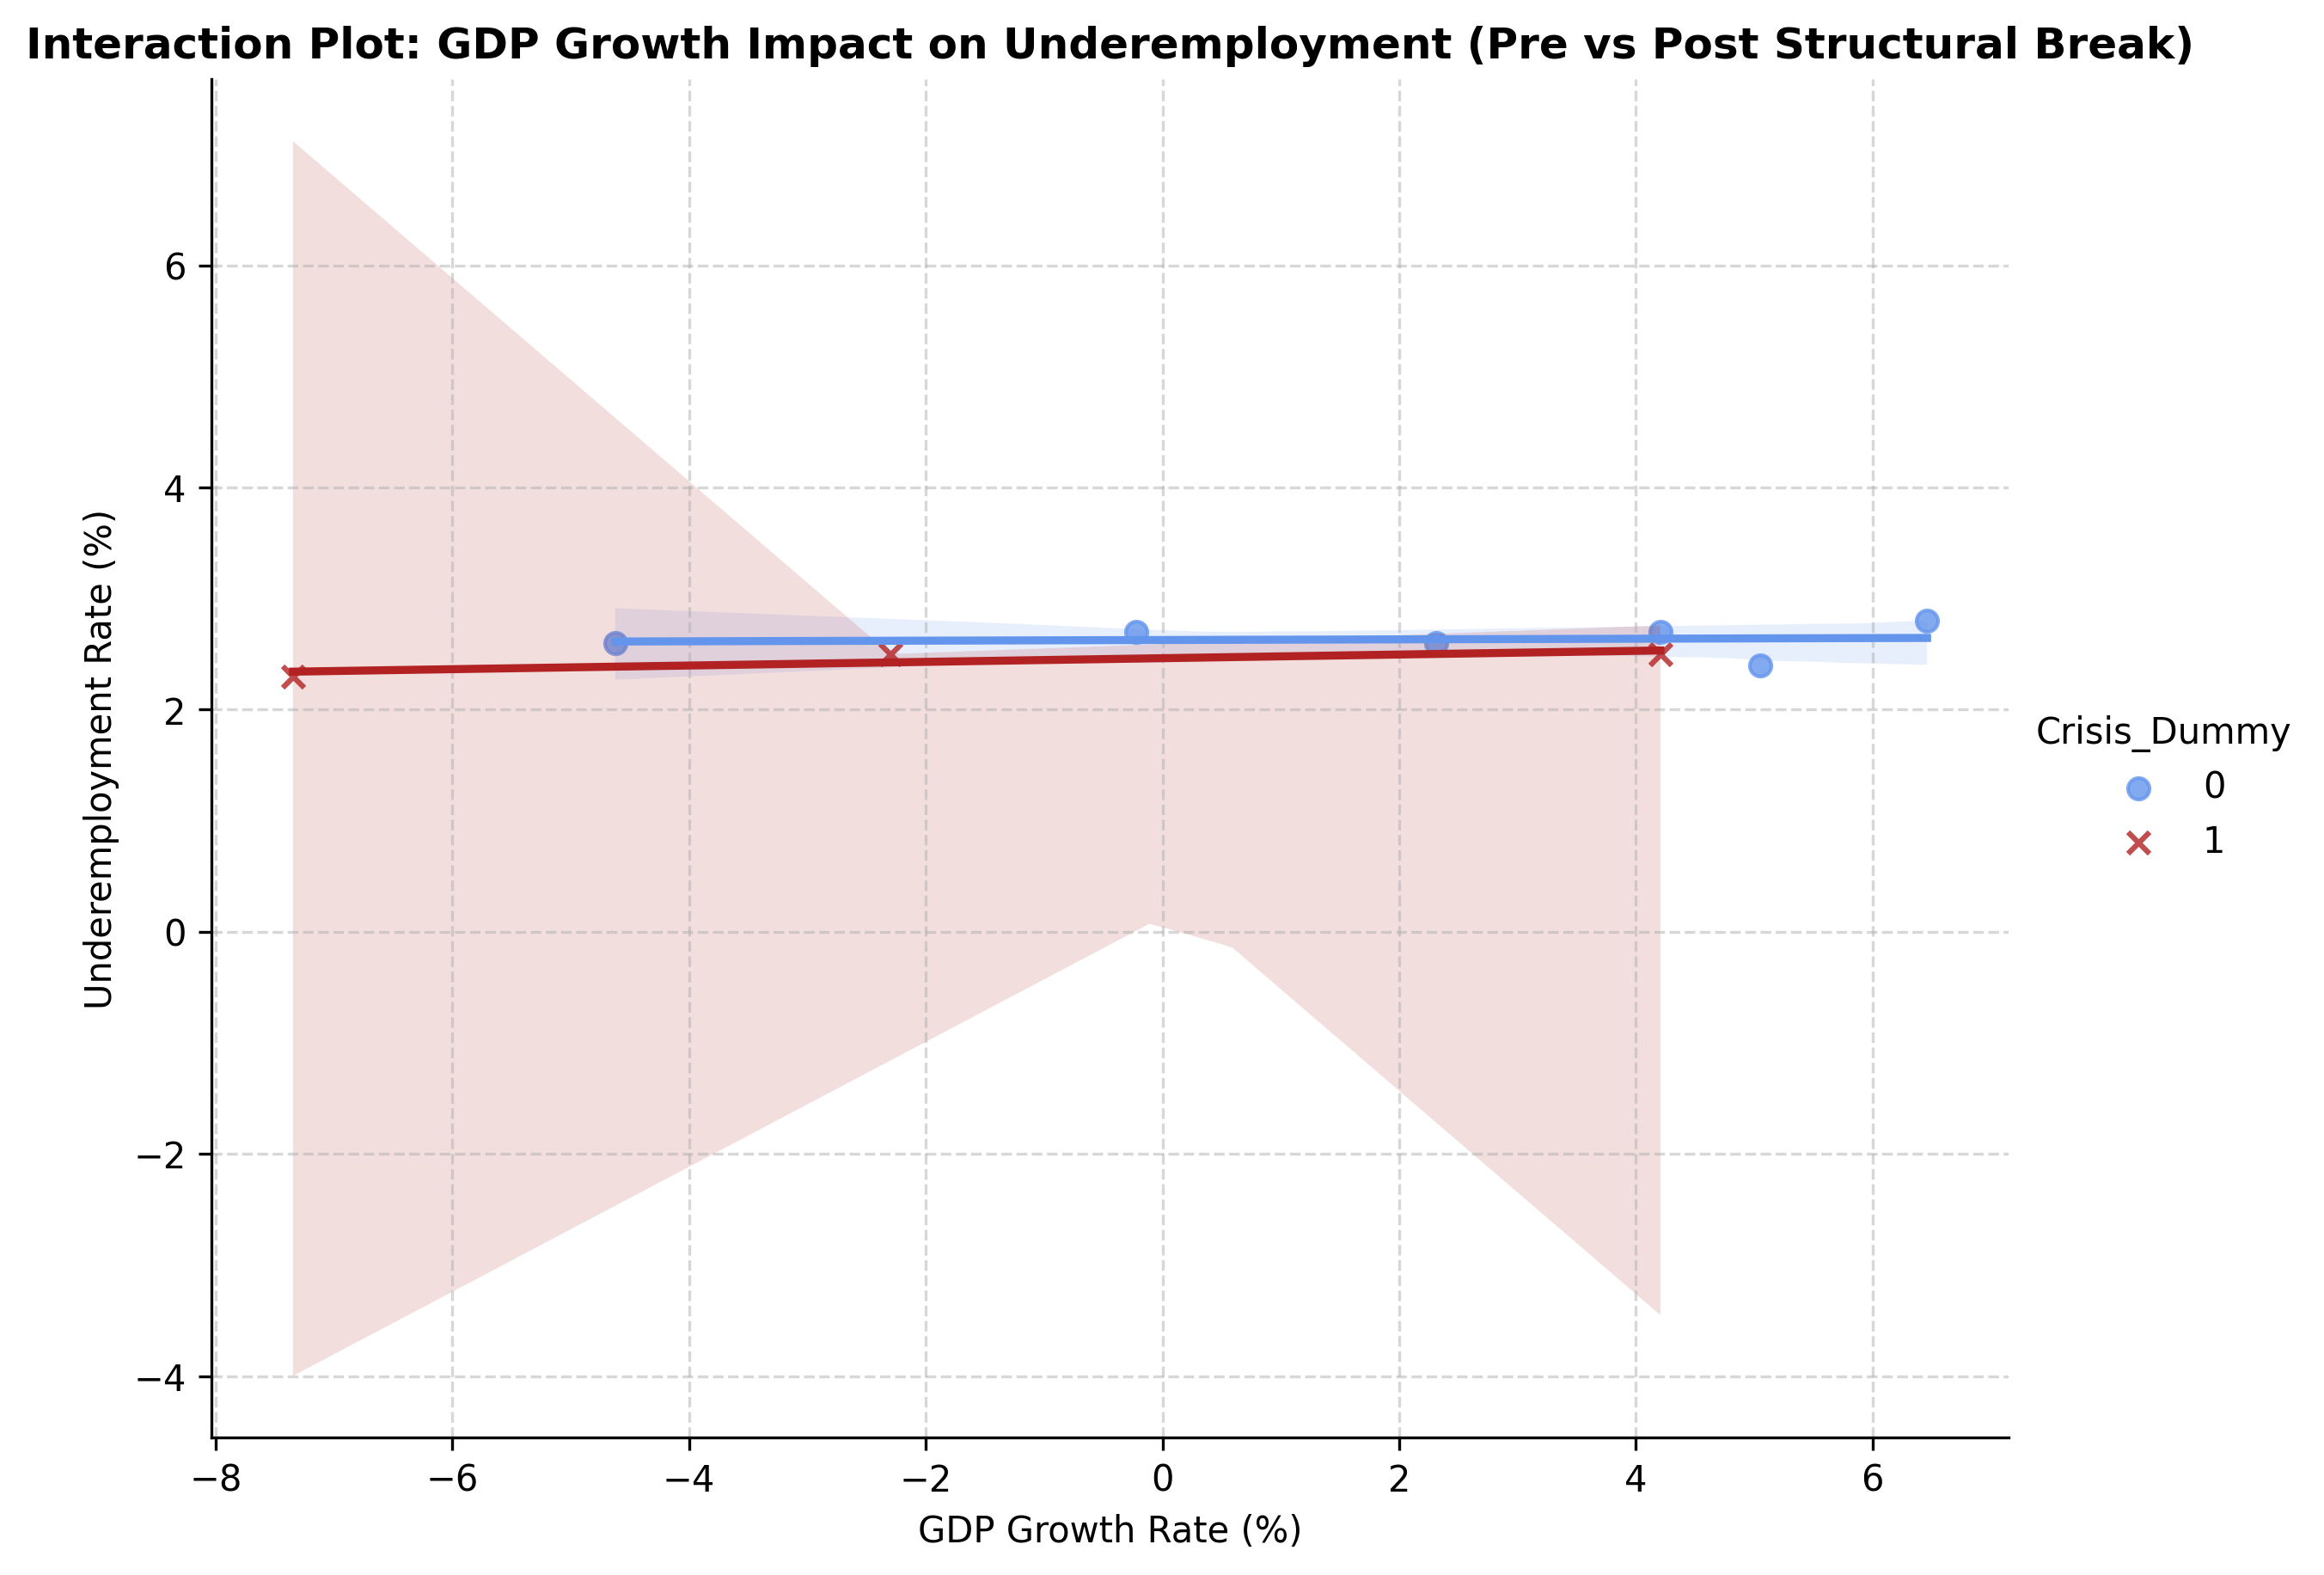
\includegraphics[width=\linewidth, height=3.2cm, keepaspectratio]{GDP_Interaction_Break.png}
  \caption{GDP Growth $\times$ Crisis interaction. Blue: pre-break slope;
    red: post-2022 slope. Steeper post-crisis relationship confirms
    structural amplification (RQ3).}
  \label{fig:interaction}
\end{figure}

\subsection{Lagged Dependencies (RQ2, RQ4)}

Figure~\ref{fig:tlcc} shows GDP and inflation shocks lagging 2--3 quarters
before realising in underemployment, consistent with labour market
hysteresis. This informs the XGBoost lag features and provides directional
support for long-run cointegration. Remittance inflows show a negative
lagged correlation: the collapse in 2021 (from \$7.0~bn to \$5.5~bn as
diaspora households depleted savings) preceded the peak underemployment
quarter, consistent with remittances partially cushioning labour market
slack in normal years.

\begin{figure}[h]
  \centering
  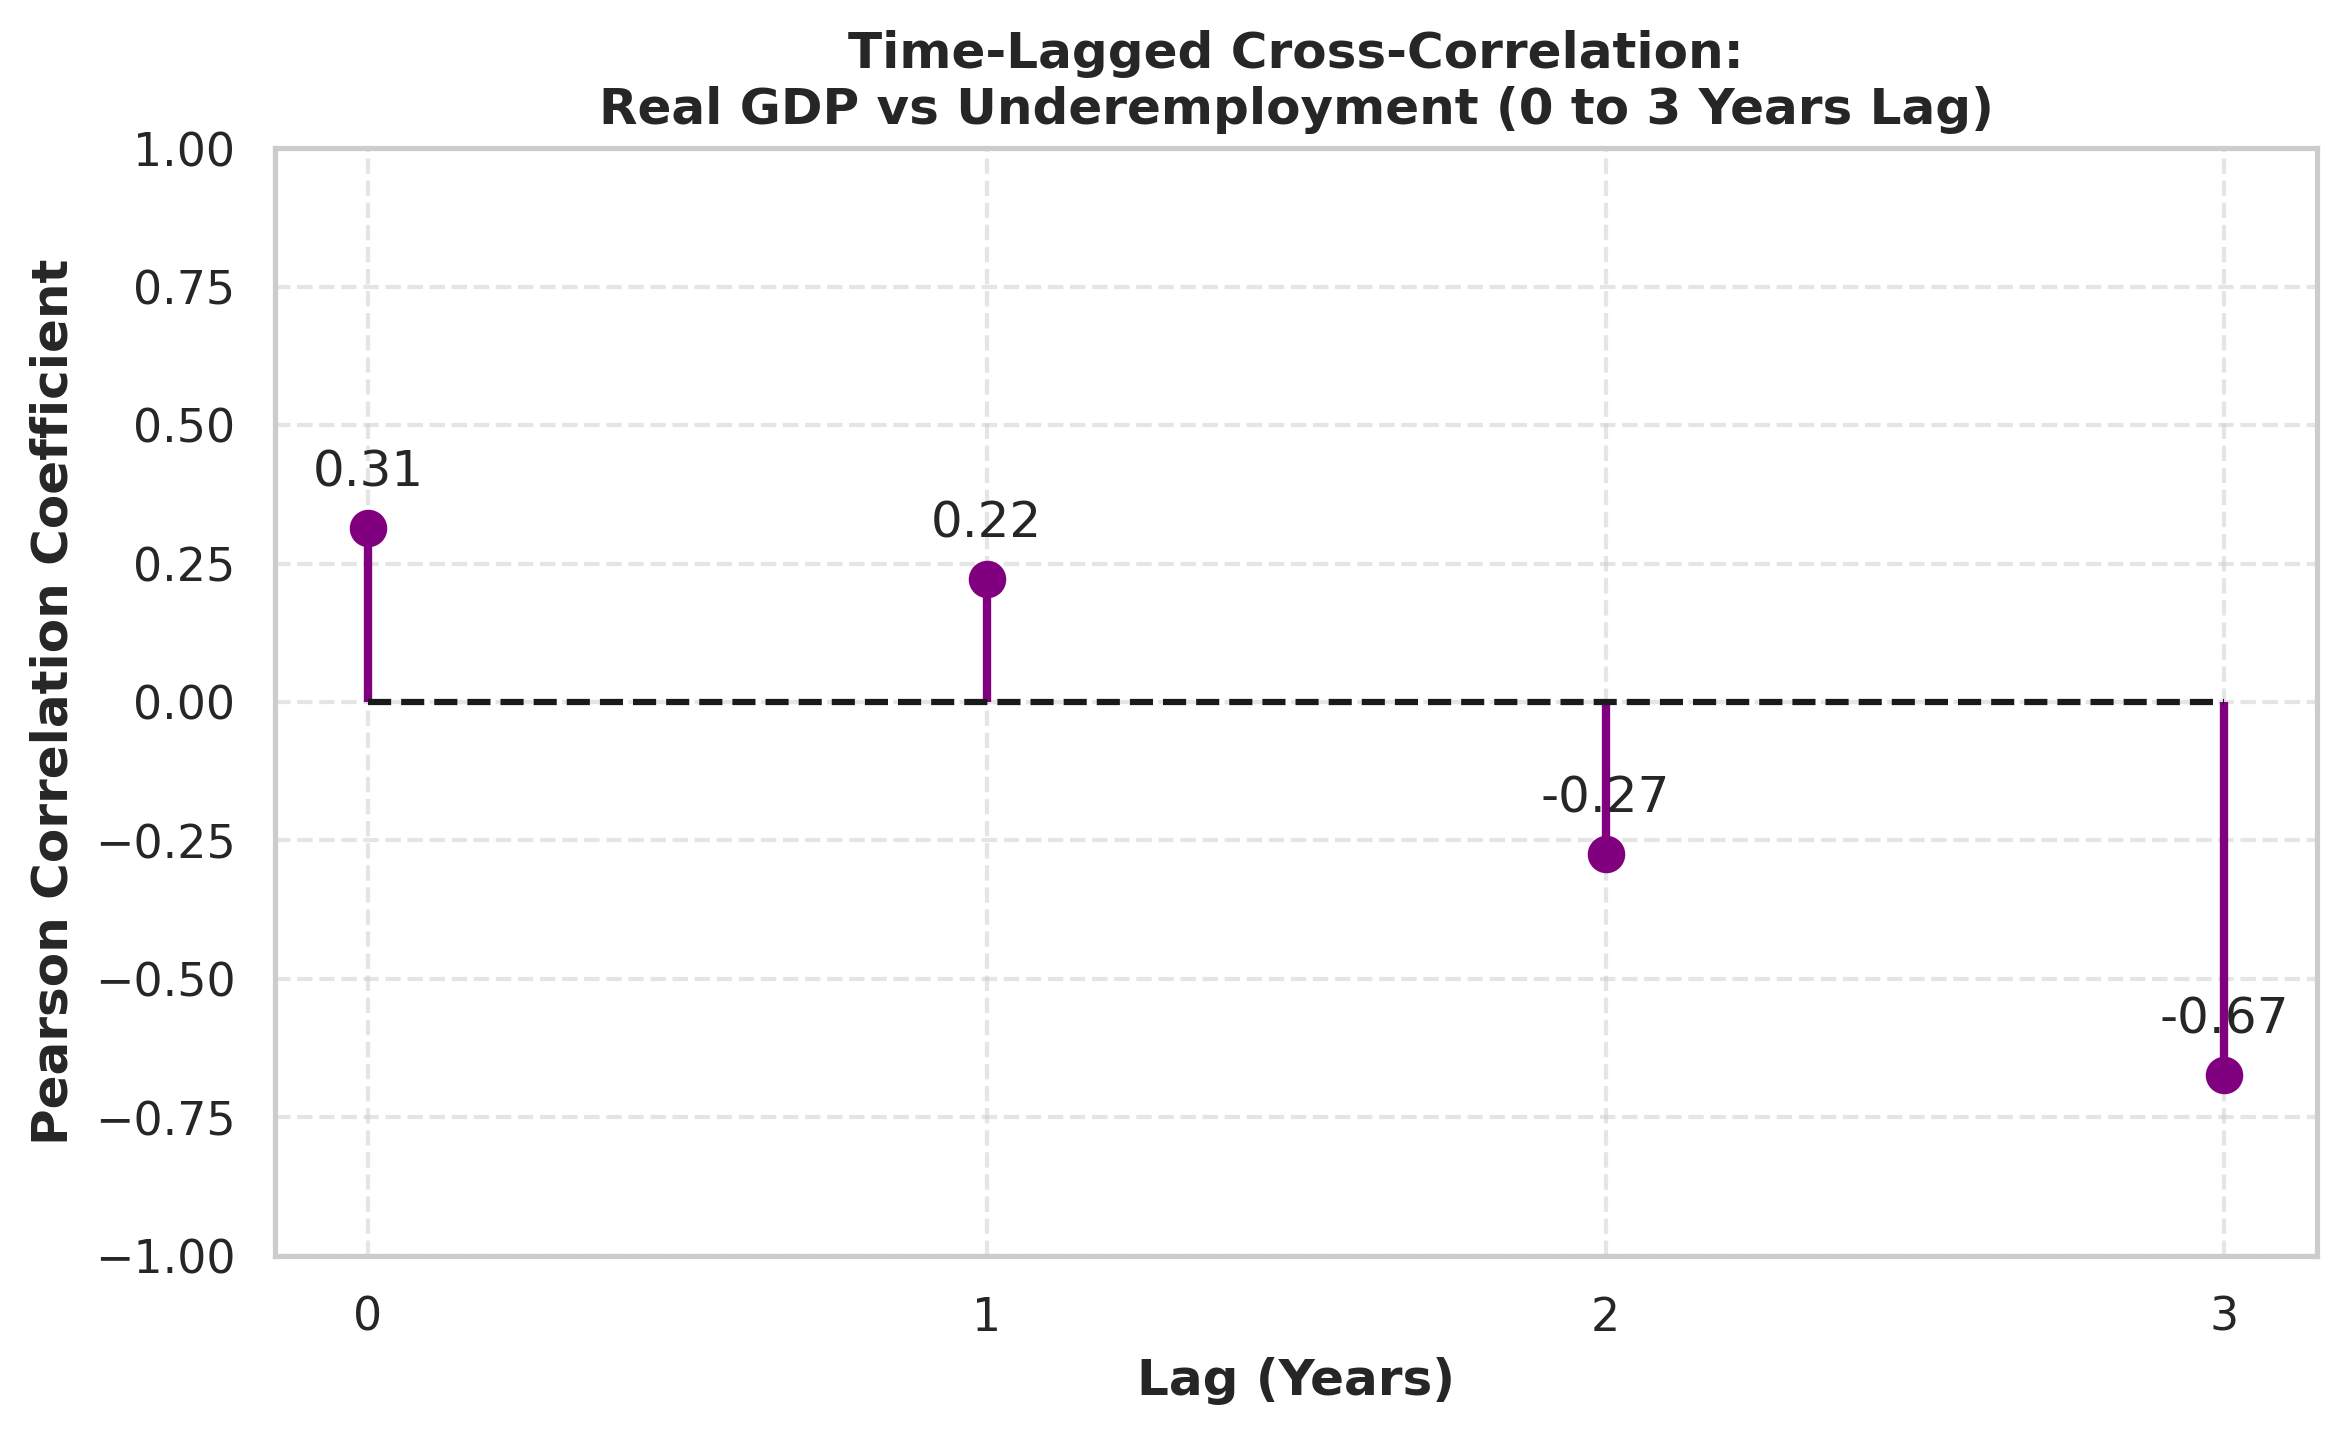
\includegraphics[width=\linewidth, height=3.2cm, keepaspectratio]{Lagged_Correlation_TLCC.png}
  \caption{TLCC matrix. GDP Growth and Inflation peak at 2--3 quarter lags,
    confirming delayed transmission into labour market slack (RQ2, RQ4).}
  \label{fig:tlcc}
\end{figure}

\subsection{SHAP Feature Association (RQ2)}

Figure~\ref{fig:shap} presents SHAP results across all nine predictors.
\textbf{(1) GDP Growth} retains the highest mean absolute SHAP value,
acting as the primary demand-side catalyst. \textbf{(2) Informal
Employment} is now the second-ranked driver, displacing inflation in the
expanded model---reflecting that the structural shift toward informal work
pre-dating the crisis amplifies underemployment independently of
price-level shocks. \textbf{(3) Youth LFPR} and \textbf{Remittances}
capture the qualification-mismatch and income-support channels respectively.
\textbf{(4)} All top SHAP directions agree with OLS coefficient signs,
providing cross-method validation.

\begin{figure}[h]
  \centering
  
\includegraphics[width=\linewidth, height=3.2cm, keepaspectratio]{shap_summary_plots.png}
  \caption{SHAP summary of model behavior. Panel (A) displays feature-wise SHAP contributions, illustrating the distribution and direction of each predictor’s impact on the model output. Panel (B) presents mean absolute SHAP values, ranking features by overall importance, with inflation emerging as the dominant driver followed by real GDP and CPI. Panel (C) shows model residuals against predicted rates, indicating no strong systematic bias but some dispersion at higher prediction levels. Overall, inflation and price-related indicators are the primary contributors to deviations from the model baseline.
.}
  \label{fig:shap}
\end{figure}

Figure~\ref{fig:shap_waterfall} shows the SHAP waterfall decomposition for
2022---the crisis peak year---illustrating how each predictor drove
underemployment above the model's baseline prediction. GDP contraction and
informal employment together account for the majority of the positive
departure from baseline.

\begin{figure}[h]
  \centering
  
\includegraphics[width=\linewidth, height=3.2cm, keepaspectratio]{shap_waterfall_2022.png}
  \caption{SHAP waterfall chart for 2022 (crisis peak). Each bar shows
    one predictor's contribution to the departure from the model baseline.
    GDP contraction and informal employment are the dominant amplifiers.}
  \label{fig:shap_waterfall}
\end{figure}

\subsection{Sensitivity Analysis: Underemployment Definitions}
\label{sec:sensitivity}

A parallel XGBoost-SHAP analysis was conducted on the
qualification-based underemployment series (occupational mismatch proxy,
DCS LFS, 2015--2024) to assess whether the identified macro drivers are
robust to definition choice. The Spearman rank correlation between the two
SHAP importance rankings is $\rho{>}0.6$, indicating that GDP contraction
and informal employment dominate \emph{both} definitions. The
qualification-based series shows a substantially higher absolute level
(${\approx}65$--$71\%$) but a smaller proportional crisis response compared
with the hours-based series, consistent with qualification mismatch being a
structural rather than cyclical phenomenon. The gender gap is persistent in
both definitions; female underemployment exceeds male across the full period
regardless of which metric is used. These findings confirm that the
study's core policy conclusions are not an artefact of definition choice.

%% ===================================================
\section{Conclusion}
%% ===================================================

Quarterly LFS micro-data reveals crisis underemployment peaks of
32.6\%---nine times the concurrent 3.8\% unemployment rate. Structural
break tests confirm 2021--2022 as a statistically significant rupture in the
underemployment--GDP--inflation system, with macro breaks leading the labour
market break by one year. The newly incorporated variables reveal two
additional findings: informal employment broke significantly in 2017,
predating the crisis and suggesting formalisation pressure as a structural
precondition; and part-time employment spiked in 2020 under COVID, acting
as a precursor to the 2022 hours-underemployment surge. SHAP establishes
GDP contraction and informal employment as the dominant drivers, with Youth
LFPR, remittances, and part-time employment capturing complementary channels.
The sensitivity analysis confirms these rankings are convergent across
hours-based and qualification-based definitions ($\rho{>}0.6$). Aggregate
unemployment is an inadequate crisis barometer for Sri Lanka.

\textbf{Limitations.} The annual dataset ($n{=}10$) rendered full ARDL and
Johansen infeasible; results are directional pending quarterly expansion.
The 2022 LFS artefact complicates annual inference for the hours-based
series. Agricultural data ends at 2024; FAOSTAT 2025 crop indices are
not yet released. The XGBoost model achieves limited out-of-sample fit at
$n{=}10$ --- SHAP values should be interpreted as association measures,
not causal estimates.

\textbf{Future work} will: (i) finalise ARDL bounds testing on the full
quarterly dataset ($n{\approx}43$) for RQ4 long-run coefficients;
(ii) incorporate the 2025 annual LFS data upon release; and (iii) extend
the sensitivity analysis to district-level disaggregation using
Table~6.4 data.

\bibliographystyle{ACM-Reference-Format}
\bibliography{references}

\end{document}
